% IEEE-style manuscript. Compile: latexmk -pdf main.tex  (requires IEEEtran, booktabs, amsmath, graphicx)
% Every number in Sections VII-VIII is generated by scripts/research/analyze_results.py
% (tables/<experiment>/*.tex, figures/<experiment>/*.pdf); see research/results_analysis.md for traceability.
\documentclass[conference]{IEEEtran}
\usepackage{amsmath,amssymb}
\usepackage{booktabs}
\usepackage{graphicx}
\usepackage{url}
\usepackage[hidelinks]{hyperref}
\graphicspath{{figures/}}

\begin{document}

\title{Do Learnable Connectivity Gates Identify Prunable Neurons?\\
A Comparative Study of Structured Neural Network Pruning}

\author{\IEEEauthorblockN{Harnoor Singh}
\IEEEauthorblockA{Undergraduate research project\\
\url{https://github.com/Harnoor001/Self-Pruning-Network}}}

\maketitle

\begin{abstract}
Self-pruning networks attach a learnable sigmoid gate to every connection and are often
assumed to ``learn'' which neurons can be removed. We test this assumption in a
controlled comparison. Starting from an existing self-pruning multilayer perceptron
(MLP) for CIFAR-10, whose neuron score is the mean gate over a neuron's incoming
connections, we compare that score with random, $\ell_1$/$\ell_2$ magnitude,
activation, first-order Taylor and Network Slimming criteria under identical compact
architectures, fine-tuning budgets and validation-based model selection, and we measure
how well each score predicts the exact validation-loss increase caused by removing a
single neuron. We show analytically that, when a gated layer is followed by batch
normalization, the mean incoming gate of a neuron is invariant to the network function
and therefore cannot be learned as an importance signal, and that an unnormalized
$\ell_1$ gate penalty under Adam moves all gates by the same amount. Over five seeds with
30-epoch sources, the mean-incoming-gate score was below random neuron selection at every
pruning ratio and on every seed: after five fine-tuning epochs it reached $53.58\%$ test
accuracy against $57.95\%$ for random at $60\%$ of hidden units removed, and all 15
alternative criteria beat it (Holm-corrected paired $t$-test). Its scores were
anti-correlated with single-neuron removal damage. Reading the same gates on the outgoing
side, which batch normalization does not cancel, recovers the accuracy of magnitude
criteria, and any positive gate penalty removes the failure, but no gate score exceeded
the conventional criteria. A VGG-16 study is specified and implemented but was not
executed in the available CPU-only environment.
\end{abstract}

\begin{IEEEkeywords}
structured pruning, importance estimation, learnable gates, batch normalization,
reproducibility
\end{IEEEkeywords}

% ---------------------------------------------------------------------------
\section{Introduction}
Structured pruning removes whole neurons or channels and, unlike unstructured
sparsity, yields physically smaller dense tensors whose speedup can be measured on
commodity hardware~\cite{li2017filters,he2024survey}. Its central decision is an
\emph{importance criterion}: which units can be removed with the least damage.
Learnable gating is an attractive alternative to hand-designed criteria: if every
connection carries a trainable multiplicative gate, gradient descent should reveal
which parts of the network matter~\cite{louizos2018l0,lee2019snip}.

This paper evaluates one concrete instance of that idea, an existing
self-pruning MLP in which each weight $W_{ij}$ is replaced by
$W_{ij}\,\sigma(S_{ij})$ and neurons are ranked by their mean incoming gate. Rather than
proposing a new algorithm, we ask five questions: whether the learned gate score
identifies prunable neurons better than conventional criteria (RQ1, RQ2); how stable
scores and decisions are across seeds (RQ3); how methods compare on measured
parameters, MACs, size and latency (RQ4); and whether the estimated importance
agrees with the actual damage of removing a neuron (RQ5).

Our contributions are: (i) a reproducible framework that applies ten criteria to the
same source network and produces identical compact architectures for every criterion;
(ii) an audit of the existing implementation, including a gate-folding error in its
compact reconstruction (Section~\ref{sec:existing}); (iii) two elementary but
consequential observations on gate learning with batch normalization and Adam
(Section~\ref{sec:analysis}); and (iv) a reliability analysis that correlates each
criterion with exact single-unit removal damage, following the methodology of
Molchanov et al.~\cite{molchanov2019importance}.

% ---------------------------------------------------------------------------
\section{Related Work}
\textbf{Magnitude criteria.} Han et al.~\cite{han2015learning} prune small weights;
Li et al.~\cite{li2017filters} rank filters by $\ell_1$ norm. With batch normalization
(BN) incoming-weight norms are scale-ambiguous~\cite{ye2018rethinking,ioffe2015bn}.
\textbf{Data-driven criteria.} Activation statistics~\cite{hu2016trimming}, first-order
Taylor expansions of the loss~\cite{molchanov2017pruning,molchanov2019importance},
activation variance~\cite{berisha2025variance} and reconstruction of the next layer
(ThiNet~\cite{luo2017thinet}) use calibration data. Recent work optimizes structures under
measured latency constraints~\cite{sun2025mdp} or at finer-than-filter group
granularity~\cite{zhang2025flexible}.
\textbf{Learned scales and gates.} Network Slimming~\cite{liu2017slimming} imposes an
$\ell_1$ penalty on BN scaling factors; $L_0$ regularization learns stochastic
gates~\cite{louizos2018l0}; SNIP scores connections through multiplicative indicator
variables~\cite{lee2019snip}. SNACS aggregates connection-level scores between filters
into structured decisions~\cite{ganesh2024snacs}; CoNNect regularizes for input--output
connectivity~\cite{franssen2025connect}. \textbf{Dependencies and dynamic pruning.}
DepGraph groups coupled parameters for arbitrary architectures~\cite{fang2023depgraph};
Probe Pruning prunes dynamically per batch~\cite{le2025probe}, a regime outside our
static scope. \textbf{Evaluation practice.} Blalock et al.~\cite{blalock2020state} and
Liu et al.~\cite{liu2019rethinking} show that unequal training budgets and single runs
can invalidate pruning comparisons; our protocol follows their recommendations.

% ---------------------------------------------------------------------------
\section{The Existing Self-Pruning Method}\label{sec:existing}
\textbf{Architecture.} The MLP maps a flattened $3072$-dimensional image through hidden
layers of widths $2048$, $1024$, $512$ to $10$ logits. Each hidden layer is
Linear$\to$BN$\to$GELU$\to$Dropout$(0.3)$.

\textbf{Gates.} Every linear layer $l$ has weights $W_l\in\mathbb{R}^{n_l\times n_{l-1}}$
(row $j$ = incoming connections of neuron $j$), an ungated bias $b_l$ and gate scores
$S_l$ of the same shape, initialized to $2$ ($\sigma(2)\approx0.881$):
\begin{equation}
h_l = (W_l \odot \sigma(S_l))\,x_{l-1} + b_l .
\end{equation}

\textbf{Objective.} With label-smoothed cross-entropy $\mathcal{L}_{\mathrm{CE}}$,
\begin{equation}
\mathcal{L} = \mathcal{L}_{\mathrm{CE}} + \lambda \sum_l \sum_{i,j}\sigma(S_{l,ji}),
\end{equation}
an unnormalized $\ell_1$ penalty over all $8.9$M gates, optimized with AdamW over all
parameters (gate scores included) for five epochs.

\textbf{Structured pruning.} The importance of hidden neuron $j$ in layer $l$ is the mean
of its \emph{incoming} gates,
\begin{equation}
I^{\mathrm{in}}_{l,j} = \frac{1}{n_{l-1}}\sum_{i}\sigma(S_{l,ji}),
\end{equation}
and each hidden layer keeps its $n_l-\lfloor r\,n_l\rfloor$ highest-scoring neurons for
a removal ratio $r$. Rows of $W_l$, $b_l$ and the BN parameters and the corresponding
columns of $W_{l+1}$ are sliced into a smaller dense network, which is then
fine-tuned.

\textbf{Audit.} The reconstruction copied $W_l$ instead of the effective weight
$W_l\odot\sigma(S_l)$, so the compact model differed from its source even at $r=0$
(validation accuracy $51.74\%\to50.70\%$ on the seed-42 checkpoint;
\texttt{research/INITIAL\_AUDIT.md}). We fold gates before slicing in all experiments
below; the legacy behavior is retained only for reproducing old artifacts.

% ---------------------------------------------------------------------------
\section{Two Properties of Gate Learning}\label{sec:analysis}
\textbf{Batch-norm invariance of incoming gates.} Let neuron $j$'s pre-activation be
$h_j=\sum_i W_{ji} g_{ji} x_i + b_j$ with gates $g_{ji}=\sigma(S_{ji})$, followed by
BN. Replacing $g_{j\cdot}$ by $c\,g_{j\cdot}$ for any $c>0$ scales the centred
pre-activation $h_j-\mathbb{E}_B[h_j]$ by $c$ (the bias cancels in the centring) and its
batch standard deviation by $c$, so the BN output is unchanged up to the
$\epsilon$ term. Hence the overall level of a neuron's incoming gates---exactly what
$I^{\mathrm{in}}$ measures---does not affect the training-mode function and receives no
consistent gradient. The argument is a direct consequence of BN's scale
invariance~\cite{ioffe2015bn} (cf.\ \cite{ye2018rethinking} for weight norms); a unit test
in our repository verifies it numerically. Outgoing gates $g_{kj}$ in layer $l+1$ scale
neuron $j$'s contribution to every downstream pre-activation and are not cancelled.
This motivates two variants evaluated separately from the existing method: the mean
outgoing gate $I^{\mathrm{out}}_{l,j}=\operatorname{mean}_k \sigma(S_{l+1,kj})$ and their
mean-normalized sum $I^{\mathrm{comb}}=I^{\mathrm{in}}/\overline{I^{\mathrm{in}}}+
I^{\mathrm{out}}/\overline{I^{\mathrm{out}}}$.

\textbf{Uniform drift under Adam.} The penalty gradient
$\partial(\lambda\sigma(S))/\partial S=\lambda\sigma'(S)$ is identical for gates with
equal scores. When it dominates the data gradient, Adam's per-coordinate normalization
makes every gate take the same step. In the committed $\lambda=10^{-3}$ checkpoint, all
hidden-layer gates lie in $[0.7417, 0.7431]$ after training, consistent with this
mechanism; with $\lambda=0$ the neuron scores span only $[0.8798, 0.8808]$ in the first
layer. These are the gates whose rankings Method~6 relies on.

\textbf{Relation to Taylor saliency.} For a gated connection,
$\partial\mathcal{L}/\partial g = W\,\partial\mathcal{L}/\partial(Wg)$, so
$g\,\partial\mathcal{L}/\partial g$ is the first-order Taylor change of the loss when the
connection is removed; gate training integrates (a sign-normalized version of) this
SNIP-like saliency~\cite{lee2019snip,molchanov2019importance}.

% ---------------------------------------------------------------------------
\section{Experimental Setup}\label{sec:setup}
\textbf{Data.} CIFAR-10~\cite{krizhevsky2009cifar}: 45{,}000/5{,}000 train/validation and
the 10{,}000-image test set, used only for final reporting. The research protocol uses a
split fixed across seeds; the verification experiment reproduces each legacy
checkpoint's own seed-dependent split exactly so that validation images were never
trained on. Activation and Taylor scores use the first 2{,}048 training images without
augmentation.

\textbf{Sources.} For each seed, the \emph{dense} source is trained with
$\mathcal{L}_{\mathrm{CE}}$ only, the \emph{gated} source with the existing objective,
and the \emph{Slimming} source with $\mathcal{L}_{\mathrm{CE}}+10^{-4}\sum|\gamma|$.
All three share the same initialization for a given seed and are trained for 30 epochs
(AdamW, learning rate $8\times10^{-4}$, cosine schedule, label smoothing $0.05$); the
best-validation epoch is kept. The gated source uses $\lambda=0$, the setting of the
existing checkpoints; other penalties are studied in ablation A. Seeds are 42, 123, 2024,
7 and 21. Compact models are fine-tuned for 5 epochs (AdamW, $2\times10^{-4}$, cosine).
In the verification experiment (Section~\ref{sec:legacy}) the dense and gated sources are
instead the committed 5-epoch checkpoints, fine-tuned for one epoch.

\textbf{Common pruning protocol.} All post-training criteria score the \emph{same} gated
source (with gates folded into the weights), and are repeated on the dense source to
isolate the training objective. Uniform allocation removes $\lfloor r n_l\rfloor$ units
per layer, $r\in\{0.2,0.4,0.6\}$, so every criterion produces the same architecture.
Every compact model is fine-tuned with the identical optimizer, schedule, budget and data
order; the checkpoint with the best validation accuracy (including the un-fine-tuned
model) is reported. An \emph{unpruned + fine-tuning} control receives the same budget so
that extra training is not credited to pruning~\cite{liu2019rethinking}.

\textbf{Reliability.} For 64 randomly sampled units per layer we zero the unit's output
(exactly equivalent to removing it, in evaluation mode; verified by tests), record the
increase of validation loss, and compute Spearman's $\rho$ between this damage and each
criterion's score, per layer and averaged over layers.

\textbf{Statistics.} We report mean $\pm$ sample standard deviation over seeds and
95\% $t$-intervals. Paired comparisons against the existing method use matched seeds
with a paired $t$-test and an exact Wilcoxon signed-rank test, Holm-corrected within each
ratio~\cite{holm1979}. With $n=3$ seeds the smallest attainable two-sided Wilcoxon $p$ is
$0.25$; we therefore treat all differences as descriptive unless the Holm-adjusted
$t$-test gives $p<0.05$, and we state the normality assumption explicitly.

% ---------------------------------------------------------------------------
\section{Baseline Methods}
Let $W_l[j]$ be neuron $j$'s incoming weights and $W_{l+1}[:,j]$ its outgoing weights
(all kernel elements for convolutions), $a_j$ its post-activation output, and
$\bar{\cdot}$ a layer mean.
\begin{align}
I^{\ell_p}_{j} &= \frac{\|W_l[j]\|_p}{\overline{\|W_l[\cdot]\|_p}}+
\frac{\|W_{l+1}[:,j]\|_p}{\overline{\|W_{l+1}[:,\cdot]\|_p}},\quad p\in\{1,2\},\\
I^{\mathrm{act}}_{j} &= \mathbb{E}_x\,\mathrm{mean}_{\mathrm{sp}}|a_j(x)|,\\
I^{\mathrm{Taylor}}_{j} &= \mathbb{E}_x\Big|\textstyle\sum_{\mathrm{sp}}a_j(x)\,
\partial\mathcal{L}(x)/\partial a_j(x)\Big|,\\
I^{\mathrm{slim}}_{j} &= |\gamma_{l,j}| \text{ (on the Slimming source)},
\end{align}
plus random scores and $|\gamma|$ on non-Slimming sources as a diagnostic. Slimming is
also reported with its original global ranking at the same total unit budget.

% ---------------------------------------------------------------------------
\section{Results and Discussion}\label{sec:results}
% Generated from artifacts/research/mlp/analysis/{findings.md,summary.csv,paired_tests.csv,
% reliability_summary.csv,stability_summary.csv,ablation_a_summary.csv,
% ablation_a_gate_statistics.csv}, artifacts/research/mlp/benchmark/benchmark_results.csv,
% and (Section~\ref{sec:legacy}) artifacts/research/mlp_legacy_sources/.
% Every number below is traceable to those files (see research/results_analysis.md).

\textbf{Executed experiments.} The main study follows the research protocol
(\texttt{configs/mlp.yaml}): 30-epoch dense, gated ($\lambda=0$) and Slimming sources
for five seeds, 5 fine-tuning epochs for every compact model, and ablations A and C on
three seeds. All of it ran on CPU (23\,h). The sources reach $60.06\pm0.17$ (dense),
$60.14\pm0.16$ (gated) and $59.51\pm0.08\%$ (Slimming) test accuracy.
Section~\ref{sec:legacy} summarizes the earlier verification on the original 5-epoch
checkpoints. The VGG-16-BN study was not executed (no GPU).

\subsection{Pruning accuracy (RQ1, RQ2)}
Table~\ref{tab:mlp_main} and Fig.~\ref{fig:acc} show test accuracy after fine-tuning.
The existing gate-in score gives the lowest accuracy of all criteria at every ratio:
$58.26$, $56.29$ and $53.58\%$ at $20$, $40$ and $60\%$ removal, against $59.98$, $59.22$
and $57.95\%$ for random selection on the same source. Before fine-tuning the gap is
larger: $44.8$/$30.5$/$18.9\%$ for gate-in against $57.4$/$46.9$/$24.0\%$ for random
(Fig.~\ref{fig:recovery}). All 15 alternative criteria beat gate-in on all five seeds at
every ratio, by $+1.2$ to $+2.2$\,pp at $20\%$, $+2.9$ to $+3.7$\,pp at $40\%$ and
$+4.4$ to $+5.3$\,pp at $60\%$. The Holm-corrected paired $t$-test supports every one of
these 45 differences at $p<0.05$ (largest adjusted $p$: $0.0046$ at $20\%$). With five
pairs the exact Wilcoxon test cannot fall below $p=0.0625$ and reaches that floor for
every comparison; Shapiro--Wilk rejects normality of the differences for 4 of the 45
comparisons, all at $20\%$.

The separately implemented gate variants, mean outgoing gate (V1) and the combined score
(V2), reach the level of the magnitude criteria (e.g.\ $58.72$ and $58.66\%$ at $60\%$,
against $58.82\%$ for $\ell_1$ and Taylor). This is consistent with
Section~\ref{sec:analysis}: BN cancels a neuron's incoming-gate level but not its outgoing
gates. In layer~1 the gate-in scores have a within-layer coefficient of variation of
$\approx9\times10^{-4}$ on every seed, against $0.11$--$0.12$ for $\ell_1$ and $0.57$--$0.59$
for Taylor. We did not test differences among the other criteria and claim no ranking
among them. Descriptively, Taylor, $\ell_1$, $\ell_2$ and $|\gamma|$ lie within
$0.35$\,pp of each other, and at $20\%$ Taylor and $\ell_1$ are within $0.1$\,pp of the
unpruned + fine-tuning control ($60.46\%$). The same criterion on the dense source gives
nearly identical accuracy ($\ell_1$ at $60\%$: $58.78$ dense vs.\ $58.82\%$ gated), so
gate training at $\lambda=0$ did not make the network more prunable. Network Slimming
retains the most accuracy before fine-tuning at $40$--$60\%$, but after fine-tuning it ends
$0.25$--$1.0$\,pp below Taylor on the gated source; its own source is $0.6$\,pp weaker, so
criterion and source are confounded. Global allocation for Slimming yields different,
smaller architectures ($-32$/$-59$/$-78\%$ parameters) and is not an equal-cost comparison.

\begin{table}[t]
\centering
\caption{\texttt{mlp}: test accuracy (\%, mean $\pm$ sample SD over 5 seeds) after 5 fine-tuning epoch(s). Criteria score the gated source except Net. Slimming (own training objective); identical compact architectures per column.}
\label{tab:mlp_main}
\footnotesize
\begin{tabular}{lccc}
\toprule
Method & 20\% units removed & 40\% units removed & 60\% units removed \\
\midrule
Gate-in (existing) & 58.26 $\pm$ 0.24 & 56.29 $\pm$ 0.16 & 53.58 $\pm$ 0.28 \\
Taylor & 60.43 $\pm$ 0.24 & 59.98 $\pm$ 0.13 & 58.82 $\pm$ 0.33 \\
Activation & 60.17 $\pm$ 0.40 & 59.60 $\pm$ 0.41 & 58.37 $\pm$ 0.18 \\
L1 in+out & 60.39 $\pm$ 0.09 & 59.96 $\pm$ 0.26 & 58.82 $\pm$ 0.21 \\
L2 in+out & 60.26 $\pm$ 0.42 & 60.04 $\pm$ 0.14 & 58.63 $\pm$ 0.42 \\
Net. Slimming & 59.41 $\pm$ 0.23 & 59.27 $\pm$ 0.29 & 58.57 $\pm$ 0.19 \\
Gate-combined (V2) & 60.26 $\pm$ 0.17 & 59.68 $\pm$ 0.28 & 58.66 $\pm$ 0.21 \\
Gate-out (V1) & 60.16 $\pm$ 0.21 & 59.87 $\pm$ 0.21 & 58.72 $\pm$ 0.08 \\
Random & 59.98 $\pm$ 0.24 & 59.22 $\pm$ 0.22 & 57.95 $\pm$ 0.07 \\
\midrule
Unpruned gated + FT & \multicolumn{3}{c}{60.46 $\pm$ 0.20} \\
Unpruned dense + FT & \multicolumn{3}{c}{60.27 $\pm$ 0.23} \\
Unpruned slimming + FT & \multicolumn{3}{c}{59.76 $\pm$ 0.24} \\
\bottomrule
\end{tabular}
\end{table}

\begin{figure}[t]
\centering
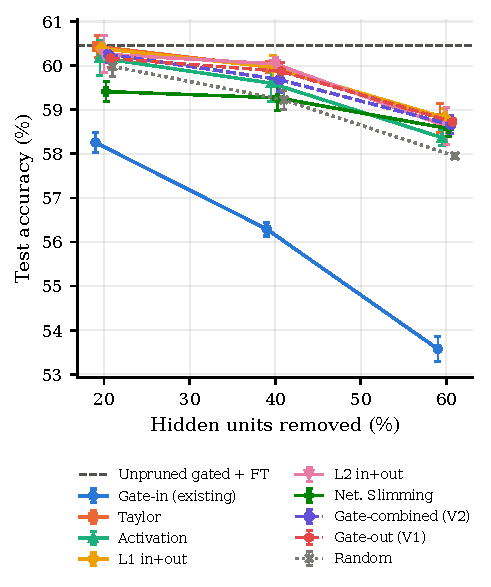
\includegraphics[width=0.85\columnwidth]{mlp/fig_accuracy_vs_ratio.pdf}
\caption{Test accuracy after five fine-tuning epochs (mean $\pm$ SD, 5 seeds; markers
offset horizontally for legibility). Dashed: unpruned gated model with the same
fine-tuning budget.}
\label{fig:acc}
\end{figure}

\begin{figure}[t]
\centering
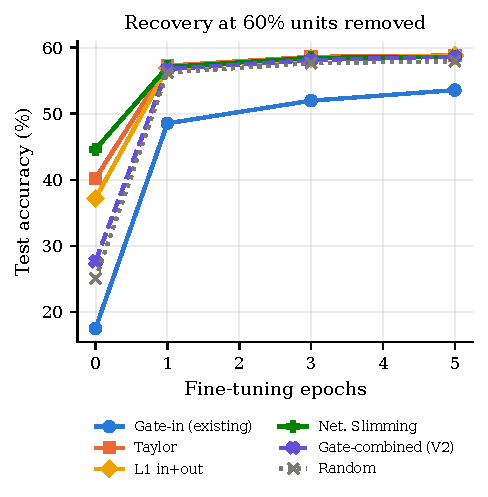
\includegraphics[width=0.85\columnwidth]{mlp/fig_finetune_recovery.pdf}
\caption{Accuracy immediately after pruning (dotted) and after fine-tuning (solid), mean
over 5 seeds.}
\label{fig:recovery}
\end{figure}

\subsection{Agreement with single-unit removal damage (RQ5)}
Fig.~\ref{fig:rel} reports Spearman's $\rho$ between each score and the validation-loss
increase caused by removing one unit (64 units per layer, 3 layers, 5 seeds). Gate-in is
the lowest criterion and negatively correlated with damage ($\rho=-0.161\pm0.088$; per
layer $-0.08$, $-0.21$, $-0.19$), below random ($-0.043\pm0.077$). On the dense and gated
sources every correlation is weak ($|\rho|\le0.17$): removing one unit changes the loss by
$1.7\times10^{-4}$ nats on average, and $23$--$24\%$ of removals \emph{decrease} it. On
the Slimming source all non-random criteria correlate more strongly with damage
($0.22$--$0.32$), and fewer removals reduce the loss ($20\%$). Taylor and activation scores
are stable under resampling of the calibration set (Spearman $0.96$--$0.99$ between two
disjoint subsets), so their weak reliability is not estimation noise. Single-unit damage
is not additive over the large groups removed in practice, so RQ5 and RQ1 measure
different properties.

\begin{figure}[t]
\centering
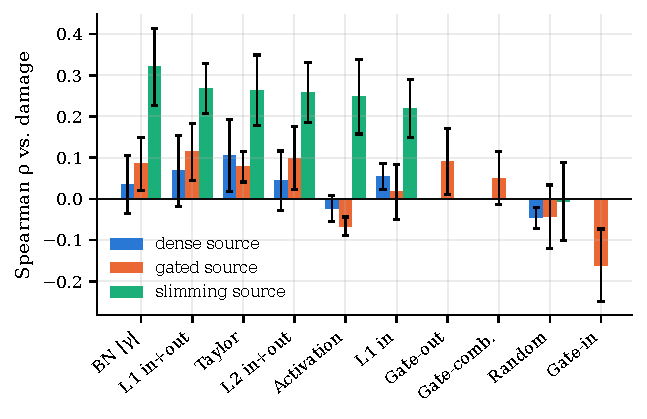
\includegraphics[width=\columnwidth]{mlp/fig_reliability_spearman.pdf}
\caption{Spearman $\rho$ between importance score and single-unit removal damage (mean
over layers, then mean $\pm$ SD over 5 seeds). Gate criteria exist only for the gated
source.}
\label{fig:rel}
\end{figure}

\subsection{Measured efficiency (RQ4)}
Uniform allocation gives identical architectures for every criterion. Deployable
parameters fall from $8.93$\,M to $6.73$, $4.73$ and $2.95$\,M ($-24.6$, $-47.0$,
$-67.0\%$), with MACs and serialized size reduced proportionally; these are physical
reductions of dense tensors. Median single-thread CPU latency at batch size 64 falls from
$11.95$\,ms to $9.47$, $6.56$ and $4.43$\,ms. Batch-1 latency also fell in this run
($1.17\to0.84$, $0.52$, $0.32$\,ms), but in the verification experiment the $20\%$ model
measured slower than dense at batch size 1, so we claim speed-ups only at batch size 64.
The gated model as trained, which recomputes $W\odot\sigma(S)$ in every forward pass,
takes $12.98$\,ms at batch size 1 ($\approx11\times$ the dense model); gates must be
folded into the weights before deployment. No GPU measurements were made.

\subsection{Verification on the original checkpoints}\label{sec:legacy}
Before the main study we evaluated the committed 5-epoch checkpoints of the existing
repository (3 seeds, $\approx52\%$ test accuracy, 1 fine-tuning epoch, each seed on its
own original split). The outcome was the same: gate-in was below random at every ratio
($47.05$ vs.\ $50.14\%$ at $60\%$), all 13 alternatives beat it on every seed, and its
scores were negatively correlated with removal damage ($\rho=-0.119\pm0.039$). Full tables
are in \texttt{research/results\_analysis.md}, Part~II.

\section{Ablation Studies}\label{sec:ablation}
The framework defines five ablations: A, gate penalty strength; B, gate aggregation
(incoming, outgoing, combined); C, fine-tuning budget; D, pruning ratio; E, seeds. B, D
and E are part of the main study above. A and C were run on seeds 42, 123 and 2024 and
are descriptive; no hypothesis tests were run on them.

\textbf{Ablation C (fine-tuning budget).} Table~\ref{tab:ablation_c} varies the budget over
$\{0,1,3,5\}$ epochs. Fine-tuning shrinks but does not close the gate-in deficit: at $60\%$
removal its gap to random is $7.5$, $7.7$, $5.7$ and $4.4$\,pp after $0$, $1$, $3$ and $5$
epochs. The other methods gain at most $0.55$\,pp from 3 to 5 epochs, so the main
budget is close to saturation for them. Without fine-tuning, Network Slimming is best at
$40$ and $60\%$, but not after five epochs. Method rankings therefore depend on the
fine-tuning budget, which is why the budget is identical for every method.

\begin{table}[t]
\centering
\caption{Ablation C: mean test accuracy (\%) versus fine-tuning epochs. The primary budget uses all seeds; the other budgets use the seeds on which ablation C was run (see findings.md for n per cell).}
\label{tab:ablation_c}
\footnotesize
\setlength{\tabcolsep}{4pt}
\begin{tabular}{llcccc}
\toprule
Method & Removed & 0 ep & 1 ep & 3 ep & 5 ep \\
\midrule
Gate-combined (V2) & 20\% & 55.40 & 59.09 & 60.38 & 60.26 \\
Gate-combined (V2) & 40\% & 44.87 & 58.41 & 59.35 & 59.68 \\
Gate-combined (V2) & 60\% & 27.67 & 56.77 & 58.11 & 58.66 \\
Gate-in (existing) & 20\% & 45.10 & 56.38 & 57.84 & 58.26 \\
Gate-in (existing) & 40\% & 30.54 & 53.05 & 55.50 & 56.29 \\
Gate-in (existing) & 60\% & 17.53 & 48.55 & 51.97 & 53.58 \\
L1 in+out & 20\% & 57.40 & 59.24 & 60.34 & 60.39 \\
L1 in+out & 40\% & 50.11 & 58.63 & 59.67 & 59.96 \\
L1 in+out & 60\% & 37.19 & 56.92 & 58.34 & 58.82 \\
Random & 20\% & 57.67 & 59.17 & 59.99 & 59.98 \\
Random & 40\% & 47.76 & 57.83 & 59.12 & 59.22 \\
Random & 60\% & 25.03 & 56.23 & 57.66 & 57.95 \\
Net. Slimming & 20\% & 58.67 & 58.67 & 59.30 & 59.41 \\
Net. Slimming & 40\% & 55.70 & 58.40 & 59.10 & 59.27 \\
Net. Slimming & 60\% & 44.62 & 57.06 & 58.46 & 58.57 \\
Taylor & 20\% & 58.68 & 59.43 & 60.25 & 60.43 \\
Taylor & 40\% & 54.01 & 58.84 & 59.77 & 59.98 \\
Taylor & 60\% & 40.23 & 57.27 & 58.60 & 58.82 \\
\bottomrule
\end{tabular}
\end{table}


\textbf{Ablation A (gate penalty).} Table~\ref{tab:ablation_a} and
Fig.~\ref{fig:lambda} train separate gated sources with the existing penalty at
$\lambda\in\{10^{-6},\dots,10^{-3}\}$ (sum) and with a mean-normalized penalty
($\lambda\in\{0.1,1\}$), and prune $40\%$ of units. The existing method's formulation is
unchanged; only $\lambda$ varies. Three observations follow. (i) The gate-in failure is
specific to $\lambda=0$: with every positive penalty, gate-in is within $0.25$\,pp of
gate-out and gate-combined and $0.36$--$0.98$\,pp above random. The penalty creates the
spread the score needs (within-layer SD of the gate-in score $\le8\times10^{-4}$ at
$\lambda=0$, $0.025$--$0.12$ at $\lambda=10^{-6}$). (ii) Source accuracy is unaffected
($60.05$--$60.32\%$) even at $\lambda=10^{-3}$, where all connection gates have collapsed
to $\sigma(S)\approx0.087$ with a within-layer SD below $2.5\times10^{-4}$. Batch
normalization absorbs the uniform rescaling, a direct observation of both properties in
Section~\ref{sec:analysis}. (iii) Stronger sum penalties lower post-pruning accuracy for
all criteria, random included ($59.49\to57.52\%$), so they make the network harder to
prune at this budget rather than making the gates more informative. The mean-normalized
penalties show no such drop.

\begin{table}[t]
\centering
\caption{Ablation A: test accuracy (\%, mean over 3 seeds) when the gated source is trained with different gate penalties.}
\label{tab:ablation_a}
\footnotesize
\setlength{\tabcolsep}{2.5pt}
\begin{tabular}{lccccc}
\toprule
Penalty & Source & Gate-comb. & Gate-in & Gate-out & Random \\
\midrule
$\lambda$=0 & 60.25 & 59.63 & 56.30 & 59.84 & 59.27 \\
$\lambda$=1e-06 (sum) & 60.32 & 59.76 & 59.85 & 59.88 & 59.49 \\
$\lambda$=1e-05 (sum) & 60.09 & 59.18 & 59.30 & 59.35 & 58.68 \\
$\lambda$=0.0001 (sum) & 60.20 & 58.33 & 58.31 & 58.55 & 57.62 \\
$\lambda$=0.001 (sum) & 60.05 & 57.93 & 57.90 & 58.04 & 57.52 \\
$\lambda$=0.1 (mean) & 60.23 & 59.91 & 59.92 & 59.91 & 58.94 \\
$\lambda$=1 (mean) & 60.28 & 59.86 & 59.69 & 59.81 & 59.09 \\
\bottomrule
\end{tabular}
\end{table}


\begin{figure}[t]
\centering
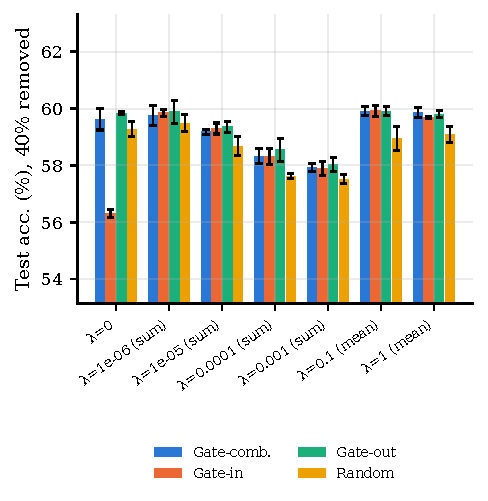
\includegraphics[width=\columnwidth]{mlp/fig_ablation_gate_lambda.pdf}
\caption{Ablation A: test accuracy after removing $40\%$ of hidden units from gated
sources trained with different penalties (mean $\pm$ SD, 3 seeds, 5 fine-tuning
epochs).}
\label{fig:lambda}
\end{figure}


% ---------------------------------------------------------------------------
\section{Limitations}
\begin{itemize}
\item \textbf{Executed scope.} The MLP study (five seeds), its ablations A and C (three
seeds) and the verification on the original checkpoints were executed on CPU. The
VGG-16-BN study is implemented and dry-run tested, but was not executed and no results are
reported for it.
\item \textbf{Model quality.} The MLP sources reach about 60\% test accuracy on raw
pixels; conclusions may differ for stronger models.
\item \textbf{Statistical power.} With five seeds the exact Wilcoxon test cannot reach
$p<0.0625$, so significance rests on the paired $t$-test, whose normality assumption is
questionable for 4 of 45 comparisons. Ablations A and C (three seeds) are descriptive.
\item \textbf{Confounds.} Network Slimming is evaluated on its own source, which is
$0.6$\,pp weaker; global allocation changes the architecture and is not an equal-cost
comparison.
\item \textbf{Hardware.} Latency was measured on one CPU with one thread; no GPU was
available, so no GPU latency or memory figures are reported.
\item \textbf{Architecture.} An MLP on raw pixels is not representative of modern
vision models; the CNN extension is required before generalizing.
\end{itemize}

\section{Conclusion}
% Conclusions are limited to the executed experiments (Section~\ref{sec:results}): the MLP
% study and the reduced-budget VGG-16-BN study.
We asked whether the learnable connection gates of an existing self-pruning MLP identify
prunable neurons. Every criterion used the same compact architectures, fine-tuning budget
and validation-based selection, over five seeds with 30-epoch sources. In the setting the
existing method ships with ($\lambda=0$) the answer is \emph{no}: its neuron score, the
mean incoming gate, gave lower accuracy than random neuron selection at every pruning ratio
and on every seed, by up to $4.4$\,pp after fine-tuning, and its scores were
anti-correlated with the measured damage of removing a neuron. The same result held on the
original 5-epoch checkpoints. This matches the analysis in Section~\ref{sec:analysis}:
behind batch normalization, the level of a neuron's incoming gates does not affect the
network function.

Three outcomes are constructive. First, reading the same gates on the outgoing side, which
BN does not cancel, recovers the accuracy of standard magnitude criteria. Second, any
positive gate penalty we tested removes the failure: gate-in then matches the other gate
scores and exceeds random selection (descriptively, three seeds). Even so, in the main study no gate score exceeded the conventional
criteria, and stronger sum penalties made the networks harder to prune for every
criterion. Third, the audit found and corrected a gate-folding error in the original
compact reconstruction. The results do \emph{not} show that gate-based criteria are better
than conventional ones, and they establish no ranking among the conventional criteria,
which were not tested against each other.

A reduced-budget VGG-16-BN study (20-epoch sources, three fine-tuning epochs, three seeds)
points in the same direction: gate-in fell below random at $40$ and $60\%$ channel removal
and lost to every other criterion on every seed at $60\%$. With three seeds, however, only
one comparison survives multiple-testing correction, so this is supporting rather than
independent evidence for convolutional networks. The main conclusions rest on one MLP
architecture on raw CIFAR-10 pixels, CPU-only measurements and three seeds for the
ablations. The full VGG-16-BN protocol (160-epoch sources, 20 fine-tuning epochs, five
seeds, gate-penalty ablation) on a GPU is the necessary next step before the findings can
be generalized.


\bibliographystyle{IEEEtran}
\bibliography{references}

\end{document}
